% !TeX root = ../Harte_Kugeln.tex
%\subsection{Sampling} % Probenentnahme? Messungsintervalle? 

\newcommand{\reffig}[1]{Abbildung \ref{fig:#1}}

Um die nächste Stoßzeit zu ermitteln genügt es, sich jeweils Zwei Kugeln anzusehen und sich deren Kollisionszeit zu berechnen. Weiß man die Kollisionszeiten aller Kugeln im System, so weiß man auch den Zeitpunkt der nächsten Kollision. Man muss also nicht das System als ganzes betrachten, es genügt das Verhalten von jeweils zwei Kugeln zu kennen.
Im Zentrum der Simulation steht somit der Algorithmus zur Erkennung ob und wann zwei Kugeln einander stoßen werden. 
Da wir eine Box mit periodischen Randbedingungen betrachten, muss der gewählte Algorithmus auch mit Kugeln am Rand der Box klarkommen. Unser Ansatz beruht auf einer Koordinatentransformation und wird in diesem Kapitel näher beschrieben.


% !TeX root = ../Harte_Kugeln.tex
\subsubsection{Kollisionsprüfung} % Probenentnahme? Messungsintervalle? 

%Parameter zur Darstellung der Box und Kugeln in diesem Absatz
\newcommand{\BoxW}{10}
\newcommand{\BoxH}{7}
\newcommand{\Kradius}{.7}

\newcommand{\Kx}{7}
\newcommand{\Ky}{6}

\newcommand{\vxa}{6/3}
\newcommand{\vya}{2/3}
\newcommand{\vxb}{-5/3}
\newcommand{\vyb}{3/3}

\newcommand{\Dx}{-2.5}
\newcommand{\Dy}{-5}

\newcommand{\BoxC}{\BoxW / 2 , \BoxH / 2}
\newcommand{\BoxWh}{\BoxW / 2}
\newcommand{\BoxHh}{\BoxH / 2}

\newcommand{\drawKugel}[1]{
    \draw[fill=black] 	(#1) circle (0.15em);
    \draw		(#1) circle (\Kradius);
}

\newcommand{\dis}{r_{21}}
\newcommand{\vdis}{\vec{r}_{21}}
\newcommand{\vdissq}{\left|\vdis\right|^2}

\newcommand{\vel}{v_{21}}
\newcommand{\vvel}{\vec{v}_{21}}
\newcommand{\vvelsq}{\left|\vvel\right|^2}
\newcommand{\dia}{d}

%\subsubsection{Koordinatentransformation}
Zur besseren Veranschaulichung wird der Algorithmus in 2 Dimensionen vorgestellt, er ist jedoch ohne Probleme auf beliebige Dimensionen erweiterbar.\\
In \reffig{Koortrans01} ist die Ausgangsposition zweier beliebiger Kugeln dargestellt. In dieser Darstellung ist eine Berechnung der Kollision erschwert da beide Kugeln ohne Kontakt und zu verschiedenen Zeiten die betrachtete Box verlassen.

% !TeX root = ../Harte_Kugeln.tex

\begin{figure}[H]
  \centering
  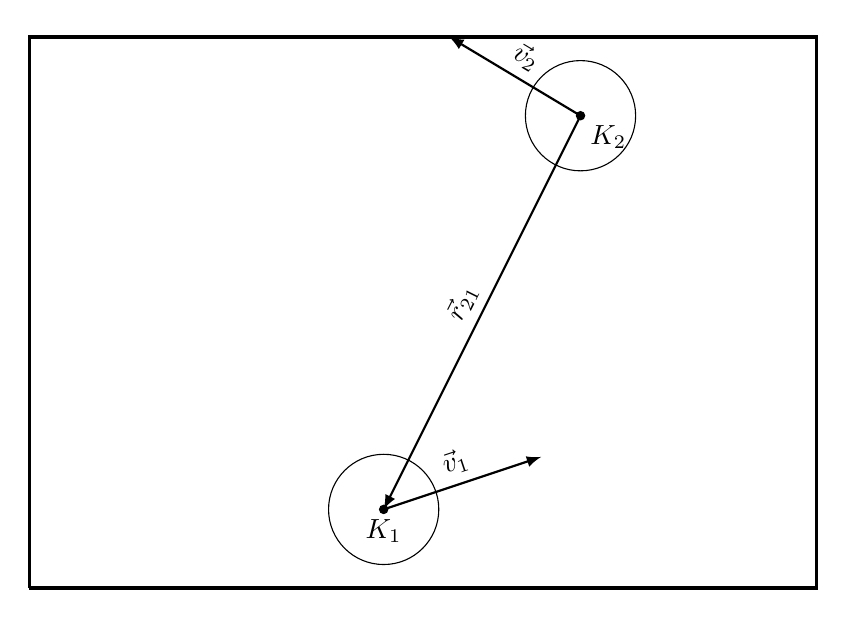
\begin{tikzpicture}
    \coordinate (Origin)   at (0,0);
    \coordinate (OL) at (0,\BoxH);
    \coordinate (OR) at (\BoxW,\BoxH);
    \coordinate (UR) at (\BoxW,0);
    
    \draw [very thick] (Origin) -- (OL) -- (OR) -- (UR) -- (Origin);
    
    \coordinate [label={below right:$K_2$}] (K2) at (\Kx,\Ky);
    \drawKugel{K2};
    
    \coordinate [label={below:$K_1$}] (K1) at (\Kx+\Dx,\Ky+\Dy);
    \drawKugel{K1};

	\draw[-latex, thick] (K2) -- (K1) node[midway,above,sloped] {$\vdis$};
	
	\draw[-latex, thick] (K1) -- (\Kx+\Dx+\vxa, \Ky+\Dy+\vya) node[midway,above,sloped] {$\vec{v}_1$};
	\draw[-latex, thick] (K2) -- (\Kx+\vxb, \Ky+\vyb) node[midway,above,sloped] {$\vec{v}_2$};
  \end{tikzpicture}
  \caption{Ausgansposition der betrachteten Kugeln.}
  \label{fig:Koortrans01}
\end{figure}





Um eine leichter zu handhabende Darstellung zu erhalten und Effekten mit Stoßpartnern am Rand unserer Box aus dem Weg zu gehen transformieren wir unser System so, dass sich eine der am berechneten Stoß beteiligten Kugeln im Zentrum der Box befindet. Da wir eine Box mit periodischen Randbedingungen gewählt haben ist dies ohne weitere Probleme möglich. In \reffig{Koortrans02} ist das Resultat einer solchen Verschiebung um Kugel 2 zu sehen.

% !TeX root = ../Harte_Kugeln.tex

\begin{figure}[H]
  \centering
  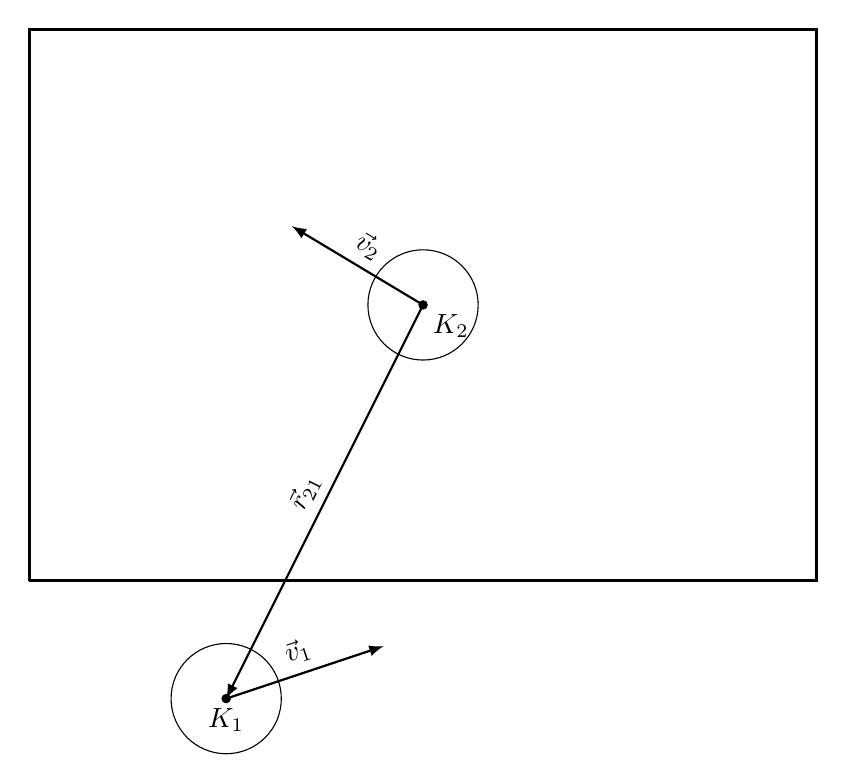
\begin{tikzpicture}
    \coordinate (Origin)   at (0,0);
    \coordinate (OL) at (0,\BoxH);
    \coordinate (OR) at (\BoxW,\BoxH);
    \coordinate (UR) at (\BoxW,0);
    
    \draw [very thick] (Origin) -- (OL) -- (OR) -- (UR) -- (Origin);
    
    \coordinate [label={below right:$K_2$}] (K2) at (\BoxC);
    \drawKugel{K2};
    
    \coordinate [label={below:$K_1$}] (K1) at (\BoxWh+\Dx,\BoxHh+\Dy);
    \drawKugel{K1};
    
	\draw[-latex, thick] (K2) -- (K1) node[midway,above,sloped] {$\vdis$};
	
	\draw[-latex, thick] (K1) -- (\BoxWh+\Dx+\vxa, \BoxHh+\Dy+\vya) node[midway,above,sloped] {$\vec{v}_1$};
	\draw[-latex, thick] (K2) -- (\BoxWh+\vxb, \BoxHh+\vyb) node[midway,above,sloped] {$\vec{v}_2$};
  \end{tikzpicture}
  \caption{Koordinatentransformation Kugel 2 ins Zentrum der Box.}
  \label{fig:Koortrans02}
\end{figure}

Da es durch die Verschiebung dazu kommen kann, dass Kugel 1 die betrachtete Box verlässt, wie in \reffig{Koortrans03} zu sehen, muss sie durch Anwendung der Randbedingungen wieder in die Box gelegt werden.

% !TeX root = ../Harte_Kugeln.tex

\begin{figure}[H]
  \centering
  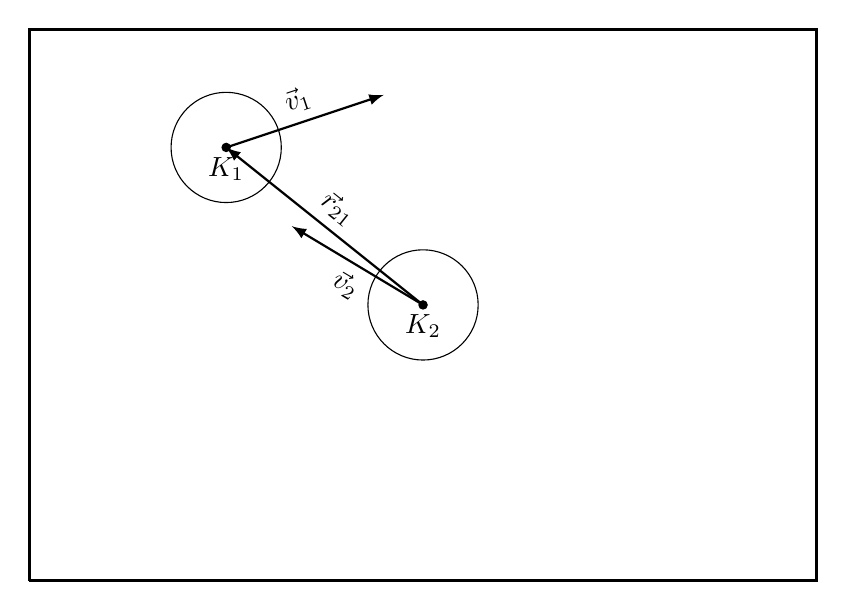
\begin{tikzpicture}
    \coordinate (Origin)   at (0,0);
    \coordinate (OL) at (0,\BoxH);
    \coordinate (OR) at (\BoxW,\BoxH);
    \coordinate (UR) at (\BoxW,0);
    
    \draw [very thick] (Origin) -- (OL) -- (OR) -- (UR) -- (Origin);
    
    \coordinate [label={below:$K_2$}] (K2) at (\BoxC);
    \drawKugel{K2};
    
    \coordinate [label={below:$K_1$}] (K1) at (\BoxWh+\Dx,\BoxHh+\Dy+\BoxH);
    \drawKugel{K1};
    
	\draw[-latex, thick] (K2) -- (K1) node[midway,above,sloped] {$\vdis$};
	
	\draw[-latex, thick] (K1) -- (\BoxWh+\Dx+\vxa, \BoxHh+\Dy+\BoxH+\vya) node[midway,above,sloped] {$\vec{v}_1$};
	\draw[-latex, thick] (K2) -- (\BoxWh+\vxb, \BoxHh+\vyb) node[midway,below,sloped] {$\vec{v}_2$};
  \end{tikzpicture}
  \caption{Kugel 1 wieder in die Box zurück gesetzt.}
  \label{fig:Koortrans03}
\end{figure}

Es ist nur Relativgeschwindigkeit der beiden Kugeln entscheidend und daher kann die Kugel im Zentrum als in Ruhe betrachten, solange sich die andere Kugeln mit der Relativgeschwindigkeit $\vvel=\vec{v}_1-\vec{v}_2$ bewegt.
 
% !TeX root = ../Harte_Kugeln.tex

\begin{figure}[H]
  \centering
  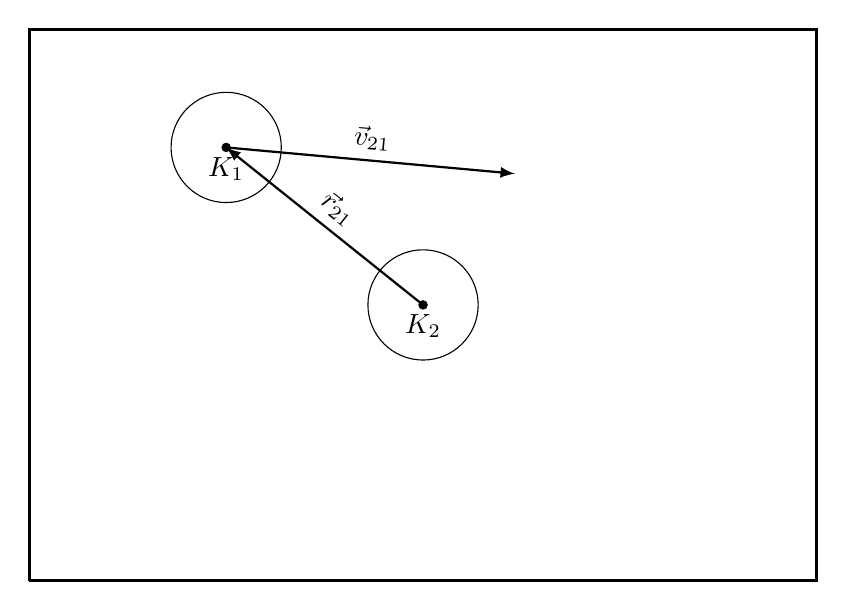
\begin{tikzpicture}
    \coordinate (Origin)   at (0,0);
    \coordinate (OL) at (0,\BoxH);
    \coordinate (OR) at (\BoxW,\BoxH);
    \coordinate (UR) at (\BoxW,0);
    
    \draw [very thick] (Origin) -- (OL) -- (OR) -- (UR) -- (Origin);
    
    \coordinate [label={below:$K_2$}] (K2) at (\BoxC);
    \drawKugel{K2};
    
    \coordinate [label={below:$K_1$}] (K1) at (\BoxWh+\Dx,\BoxHh+\Dy+\BoxH);
    \drawKugel{K1};
    
	\draw[-latex, thick] (K2) -- (K1) node[midway,above,sloped] {$\vdis$};
	
	\draw[-latex, thick] (K1) -- (\BoxWh+\Dx+\vxa-\vxb, \BoxHh+\Dy+\BoxH+\vya-\vyb) node[midway,above,sloped] {$\vvel$};
  \end{tikzpicture}
  \caption{Relativgeschwindigkeit auf Kugeln 1 übertragen.}
  \label{fig:Koortrans04}
\end{figure}

Hat man nun eine Darstellung wie in \reffig{Koortrans04} vorliegen, so kann man die Kollisionszeit durch Anwendung simpler Geometrie erhalten.
Es gilt die Abstandsgleichung 
\begin{equation}
	\vec{x} = \vdis + t\cdot\vvel
\end{equation}
mit 
\begin{equation}
	\left|\vec{x}\right| \overset{!}{=} \dia \Rightarrow \left|x\right|^2 = \dia^2
\end{equation}
zu lösen, wobei $\dia=\sigma_1/2 + \sigma_2/2$ gilt.

Somit erhält man
\begin{align}
	\dia^2	&= \left(\vdis + t\cdot\vvel \right)^2 \\
			&= \vdissq + 2t\cdot\vdis\cdot\vvel + t^2\vvelsq
\end{align}
und nach Auflösen nach der Kollisionszeit $t$
\begin{equation}
	t_{1,2}=\frac{\vdis\cdot\vvel \pm \sqrt{\left(\vdis\cdot\vvel\right)^2 - \vdissq\vvelsq + \vvelsq\dia^2}}{\vvelsq}.
\end{equation}

Die Berechnung kann noch vereinfacht werden. Wie man in \reffig{Koortrans04} sieht, kann es nur zu einer Kollision kommen wenn $\vdis\cdot\vvel < 0$ ist. Daher kann nur die Addition des Wurzelterms zu einem Ergebnis mit positiver Zeit führen.\\
Kommt es zu keinem Stoß in dieser Box, so verlässt Kugel 1 die Box und wird, entsprechend den Randbedingungen des Systems, wieder zurückgesetzt.

